% Compile with:
% latexmk -pvc -interaction=nonstopmode *Seminar.tex
\documentclass[aspectratio=169,10pt]{beamer}
\usetheme{UniBern}
\title{Tomographic imaging of fish}
\subtitle{Or how to image much, \emph{much} more teeth}
\author{David Haberthür}
\institute{Institute of Anatomy\\Universität Bern}
\date{January 18, 2024 | Seminar@Institute of Anatomy}

% Some often used abbreviations/commands
\newcommand{\everyframe}{333}% use only every nth frame for the animations
\newcommand{\imagewidth}{\columnwidth}% set global image width
\newcommand{\imageheight}{0.618\paperheight}% set global image heidht
\newlength\imagescale% needed for scalebars
\newcommand{\uct}{{\textmu}CT\xspace}% make our life easier
\newcommand{\eg}{e.\,g.\xspace}%
\newcommand{\ie}{i.\,e.\xspace}%

% \usepackage[backend=biber,
% 	url=false,
% 	isbn=false,
% 	eprint=false,
% 	sorting=none]{biblatex}


\usepackage[%
    backend=biber,
    style=ieee,
		url=false,
		isbn=false,
    citetracker=true,
    ]{biblatex}
\addbibresource{../../Documents/library.bib} % FastSSD, Windows or Mac works (on Linux/FastSSD we generated a 'Document' folder at the correct level and `ln -s ~/P/Documents/library.bib .` to it)
\usepackage{tikz}
	\usetikzlibrary{shadows,spy}
	\tikzset{shadowed/.style={preaction={transform canvas={shift={(1pt,-1pt)}},draw=ubRed}}}
\usepackage{shadowtext}
	\shadowoffset{1pt}
	\shadowcolor{ubRed}
\usepackage{pgfplots}
	\pgfplotsset{compat=newest}
\usepackage{microtype}
\usepackage[detect-all=true,
	range-phrase=--,
	range-units=single,
	per-mode=symbol,
	per-symbol=/]{siunitx}
\usepackage[absolute,overlay]{textpos}
\usepackage[showseconds=false,showzone=false]{datetime2}
\usepackage{gitinfo2}
\usepackage{xspace}
\usepackage{ccicons}
\usepackage{fontawesome5}
\usepackage[version=4]{mhchem}
\usepackage{animate}
\usepackage{listings}
	\lstset{basicstyle=\scriptsize\ttfamily}
	% highlight a line in listings: https://tex.stackexchange.com/a/58543/828
	% Including a crude workaround for recent versions of `listings`: https://tex.stackexchange.com/a/451538/828
	\makeatletter%
	\let\old@lstKV@SwitchCases\lstKV@SwitchCases%
	\def\lstKV@SwitchCases#1#2#3{}%
	\makeatother%
	\usepackage{lstlinebgrd}%
	\makeatletter%
	\let\lstKV@SwitchCases\old@lstKV@SwitchCases%
	\lst@Key{numbers}{none}{%
		\def\lst@PlaceNumber{\lst@linebgrd}%
		\lstKV@SwitchCases{#1}%
		{none:\\%
		left:\def\lst@PlaceNumber{\llap{\normalfont%
		\lst@numberstyle{\thelstnumber}\kern\lst@numbersep}\lst@linebgrd}\\%
		right:\def\lst@PlaceNumber{\rlap{\normalfont%
			\kern\linewidth{}\kern\lst@numbersep%
			\lst@numberstyle{\thelstnumber}}\lst@linebgrd}%
		}{\PackageError{Listings}{Numbers #1 unknown}\@ehc}}%
	\makeatother%
	% highlight a line in listings: https://tex.stackexchange.com/a/58543/828
\usepackage{pgfplotstable}
\usepackage{booktabs}
\usepackage{colortbl}
\usepackage{mathastext}
\usepackage{lipsum}

% change tikz font to slide font
% https://tex.stackexchange.com/a/33329/828
\usepackage[eulergreek]{sansmath}
\pgfplotsset{tick label style = {font=\sansmath\sffamily},
	every axis label = {font=\sansmath\sffamily},
	legend style = {font=\sansmath\sffamily},
	label style = {font=\sansmath\sffamily}
}

% Globally thicker lines in with tikz
% https://tex.stackexchange.com/a/206769/828
\tikzset{every picture/.style={thick}}

% Define a custom footer *with* progress bar, based on https://tex.stackexchange.com/a/59749/828
\makeatletter%
\def\progressbar@progressbar{}% the progress bar
\newcount\progressbar@tmpcounta% auxiliary counter
\newcount\progressbar@tmpcountb% auxiliary counter
\newdimen\progressbar@pbht%progressbar height
\newdimen\progressbar@pbwd%progressbar width
\newdimen\progressbar@rcircle% radius for the circle
\newdimen\progressbar@tmpdim% auxiliary dimension
\progressbar@pbwd=0.75\paperwidth%
\progressbar@rcircle=1.5pt%
\def\progressbar@progressbar{%
	\progressbar@tmpcounta=\insertframenumber%
	\progressbar@tmpcountb=\inserttotalframenumber%
	\progressbar@tmpdim=\progressbar@pbwd%
	\multiply\progressbar@tmpdim by \progressbar@tmpcounta%
	\divide\progressbar@tmpdim by \progressbar@tmpcountb%
		\hfill%
		\begin{tikzpicture}%
			\draw[ubGrey] (0,0) -- ++ (\progressbar@pbwd,0);%
			\draw[draw=ubRed,fill=ubGrey] (\the\dimexpr\progressbar@tmpdim-\progressbar@rcircle\relax,.5\progressbar@pbht) circle (\progressbar@rcircle);%
		\end{tikzpicture}%
		\hfill%
		bit.ly/ana-smnr-24\xspace|%
		\xspace v.~\href{https://github.com/habi/Talk.2024.AnatomyInternalSeminar/commit/\gitHash}{\gitAbbrevHash}\xspace|%
		\xspace p.~\insertframenumber/\inserttotalframenumber%
\vspace{0.5ex}%
}%
\addtobeamertemplate{footline}{}%
{%
	\begin{beamercolorbox}[wd=\paperwidth,center]{white}%
		\progressbar@progressbar%
	\end{beamercolorbox}%
}%
\makeatother%

% Format bibliography for beamer
% http://tex.stackexchange.com/a/10686/828
\renewbibmacro{in:}{}
% http://tex.stackexchange.com/a/13076/828
\AtEveryBibitem{%
	\clearfield{journaltitle}
	\clearfield{pages}
	\clearfield{volume}
	\clearfield{number}
	\clearname{editor}
	\clearfield{issn}
	\clearfield{year}
}%
% No parentheses around the (now empty) year: https://tex.stackexchange.com/a/147537/828
\renewcommand{\bibopenparen}{\addcomma\addspace}
\renewcommand{\bibcloseparen}{\addcomma\addspace}

% Acknowledge images just below them
% Based on https://tex.stackexchange.com/a/282637/828
\newcommand{\source}[2]{%
	% Print out (short) link under image, with small text
	\raisebox{-1.618ex}{%
		\makebox[0pt][r]{%
			\tiny\href{http://#1}{#1} #2%
			}%
		}%
	}%
\newcommand{\sourcecite}[2]{%
	% Cite (an image from) a reference
	\raisebox{-1.618ex}{%
		\makebox[0pt][r]{%
			\tiny From~\cite{#1}, #2%
			}%
		}%
	}%
\newcommand{\sourcelink}[3]{%
	% Make the source command an \href{link}{text}
	\raisebox{-1.618ex}{%
		\makebox[0pt][r]{%
			\tiny\href{#1}{#2}, #3%
			}%
		}%
	}%

% % References as footnotes at the bottom of the slides
% % https://tex.stackexchange.com/a/368760/828
% \makeatletter
% \renewcommand\@makefnmark{\xspace\hbox{\usebeamercolor[fg]{footnote mark}\usebeamerfont*{footnote mark}[\@thefnmark]}}
% \renewcommand\@makefntext[1]{\usebeamercolor[fg]{footnote mark}\usebeamerfont*{footnote mark}[\@thefnmark]\enspace\usebeamerfont*{footnote} #1}
% \makeatother

\makeatletter
\newbibmacro*{hypercite}{%
  \renewcommand{\@makefntext}[1]{\noindent\normalfont##1}%
  [\printfield{labelnumber}]\footnotetext{%
    \blxmkbibnote{foot}{%
    \printtext[labelnumberwidth]{%
      \printfield{prefixnumber}%
      \printfield{labelnumber}}%
    \addspace
    \fullcite{\thefield{entrykey}}}}}
\DeclareCiteCommand{\hypercite}%
  {\usebibmacro{cite:init}}
  {\usebibmacro{hypercite}}
  {}
  {\usebibmacro{cite:dump}}
\makeatother

% Reset footnote counter for every frame
\AtBeginEnvironment{frame}{\setcounter{footnote}{0}}
% Since we're using \footfullcite a lot, we remove most items to show from the citations, to keep the frames as clean as possible
\AtEveryCitekey{\clearfield{title}}
\AtEveryCitekey{\clearfield{journaltitle}}
% No "In:" http://tex.stackexchange.com/a/10686/828
\renewbibmacro{in:}{}
\AtEveryCitekey{\clearfield{volume}}
\AtEveryCitekey{\clearfield{number}}
\AtEveryCitekey{\clearfield{year}}
% No parentheses around the (now empty) year: https://tex.stackexchange.com/a/147537/828
\renewcommand{\bibopenparen}{\addcomma\addspace}
\renewcommand{\bibcloseparen}{\addcomma\addspace}
\AtEveryCitekey{\clearfield{pages}}
\AtEveryCitekey{\clearfield{issn}}

\begin{document}
% No footline on the title page
% http://tex.stackexchange.com/a/18829/828 helps us to achieve that
{%
	\setbeamertemplate{footline}{}%
	\begin{frame}[noframenumbering]
		\maketitle
	\end{frame}%
}

\begin{frame}
	\frametitle{Grüessech mitenang!}
	\begin{itemize}
		\item David Haberthür
		\begin{itemize}
			\item Physicist by trade
			\item \href{https://boris.unibe.ch/2619/}{PhD in high resolution imaging of the lung}, Institute of Anatomy, University of Bern, Switzerland
			\item Post-Doc I: \href{https://www.psi.ch/sls/tomcat/}{TOMCAT}, \href{https://www.psi.ch/sls/}{Swiss Light Source}, \href{https://www.psi.ch/}{Paul Scherrer Institute}, Switzerland
			\item Post-Doc II: \uct{} group, Institute of Anatomy, University of Bern, Switzerland.
		\end{itemize}
	\end{itemize}
\end{frame}

\section{Introduction}
\begin{frame}
	\frametitle{Grüessech from the \uct-group}
	\centering
	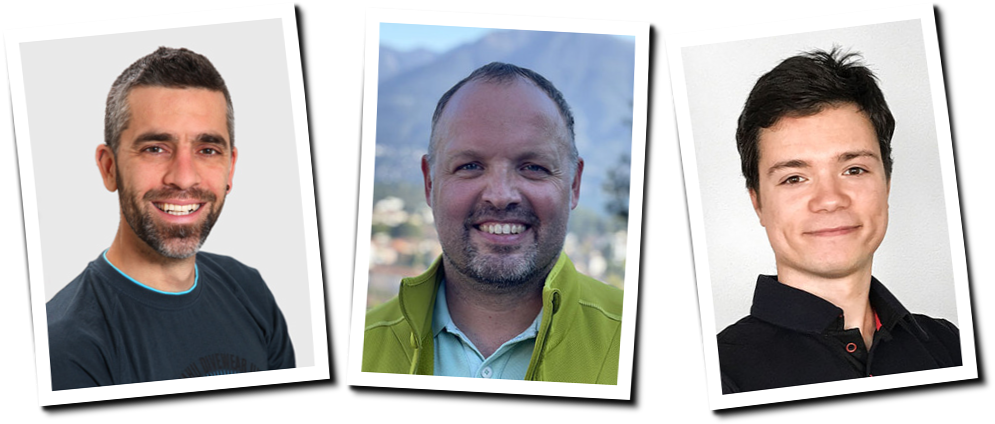
\includegraphics[height=\imageheight]{./images/team}
		\begin{columns}
		\hfill\begin{column}{0.33\textwidth}
			\centering%
			David{\color{ubRed!61.8}.}Haberthuer{\color{ubRed!61.8}@unibe.ch}%
		\end{column}
		\begin{column}{0.33\textwidth}
			\centering%
			Ruslan{\color{ubRed!61.8}.}Hlushchuk{\color{ubRed!61.8}@unibe.ch}%
		\end{column}
		\begin{column}{0.33\textwidth}
			\centering%
			Oleksiy{\color{ubRed!61.8}.}Khoma{\color{ubRed!61.8}@unibe.ch}%
		\end{column}\hfill%
	\end{columns}
\end{frame}

\renewcommand{\imagewidth}{\columnwidth}
\begin{frame}
	\frametitle{\uct-group}
	\begin{columns}
		\begin{column}{0.62\textwidth}
			\begin{itemize}
				\item microangioCT~\cite{Hlushchuk2019}
				\begin{itemize}
					\item Angiogenesis: heart, musculature~\cite{Nording2021} and bones
					\item Vasculature: (mouse) brain~\cite{Hlushchuk2020}, (human) nerve scaffolds~\cite{Wuthrich2020}, (human) skin flaps~\cite{Zubler2021} and tumors
				\end{itemize}
				\item Zebrafish musculature and gills~\cite{MesserliAaldijk2020}
				\item (Lung) tumor detection and metastasis classification~\cite{Trappetti2021}
				\item Collaborations with museums~\cite{Bochud2021} and scientist at UniBe~\cite{Halm2021,Kadlag2023} to scan a wide range of specimens, from human hearing bones to meteorites
				\item Automate \emph{all} the things!~\cite{Haberthuer2021,Haberthuer2023}
			\end{itemize}
		\end{column}%
		\begin{column}{0.38\textwidth}%
			\centering%
			\includegraphics<1>[width=\imagewidth]{./images/1172}%
			\only<1>{\source{brukersupport.com}{}}%
			\includegraphics<2>[width=\imagewidth]{./images/1272}%
			\only<2>{\source{bruker.com/skyscan1272}{}}%
			\includegraphics<3>[width=\imagewidth]{./images/2214}%
			\only<3>{\source{bruker.com/skyscan2214}{}}%
		\end{column}%
	\end{columns}%
\end{frame}


\section{Retrospection about teeth}
\begin{frame}
	\frametitle{Internal morphology of human teeth}
	\begin{columns}
		\begin{column}{0.5\textwidth}
			Collaboration with \href{https://www.zmk.unibe.ch/}{zmk bern – Zahnmedizinische Kliniken}~\hypercite{Haberthuer2021},~\hypercite{Wolf2021}
			\begin{itemize}
				\item 104 extracted human permanent mandibular canines
				\item Segmentation of teeth and root canal
				\item Numbers instead of just pretty images, unbiased characterization
				\item Reproducible and automated image analysis (\href{https://www.python.org/}{\faPython} in \href{https://jupyter.org/}{Jupyter}~\cite{Kluyver2016}
			\end{itemize}
		\end{column}%
		\begin{column}{0.5\textwidth}%
			\centering%
			\renewcommand{\imagewidth}{0.75\linewidth}
			\only<1>{%
			\pgfmathsetlength{\imagescale}{\imagewidth/2716}%
			\def\x{1678}% scalebar-x starting at golden ratio of image width of 2716px = 1678
			\def\y{2444}% scalebar-y at 90% of image height of 2716px = 2444
			\begin{tikzpicture}[x=\imagescale,y=-\imagescale]
				\node[anchor=north west, inner sep=0pt, outer sep=0pt] at (0,0) {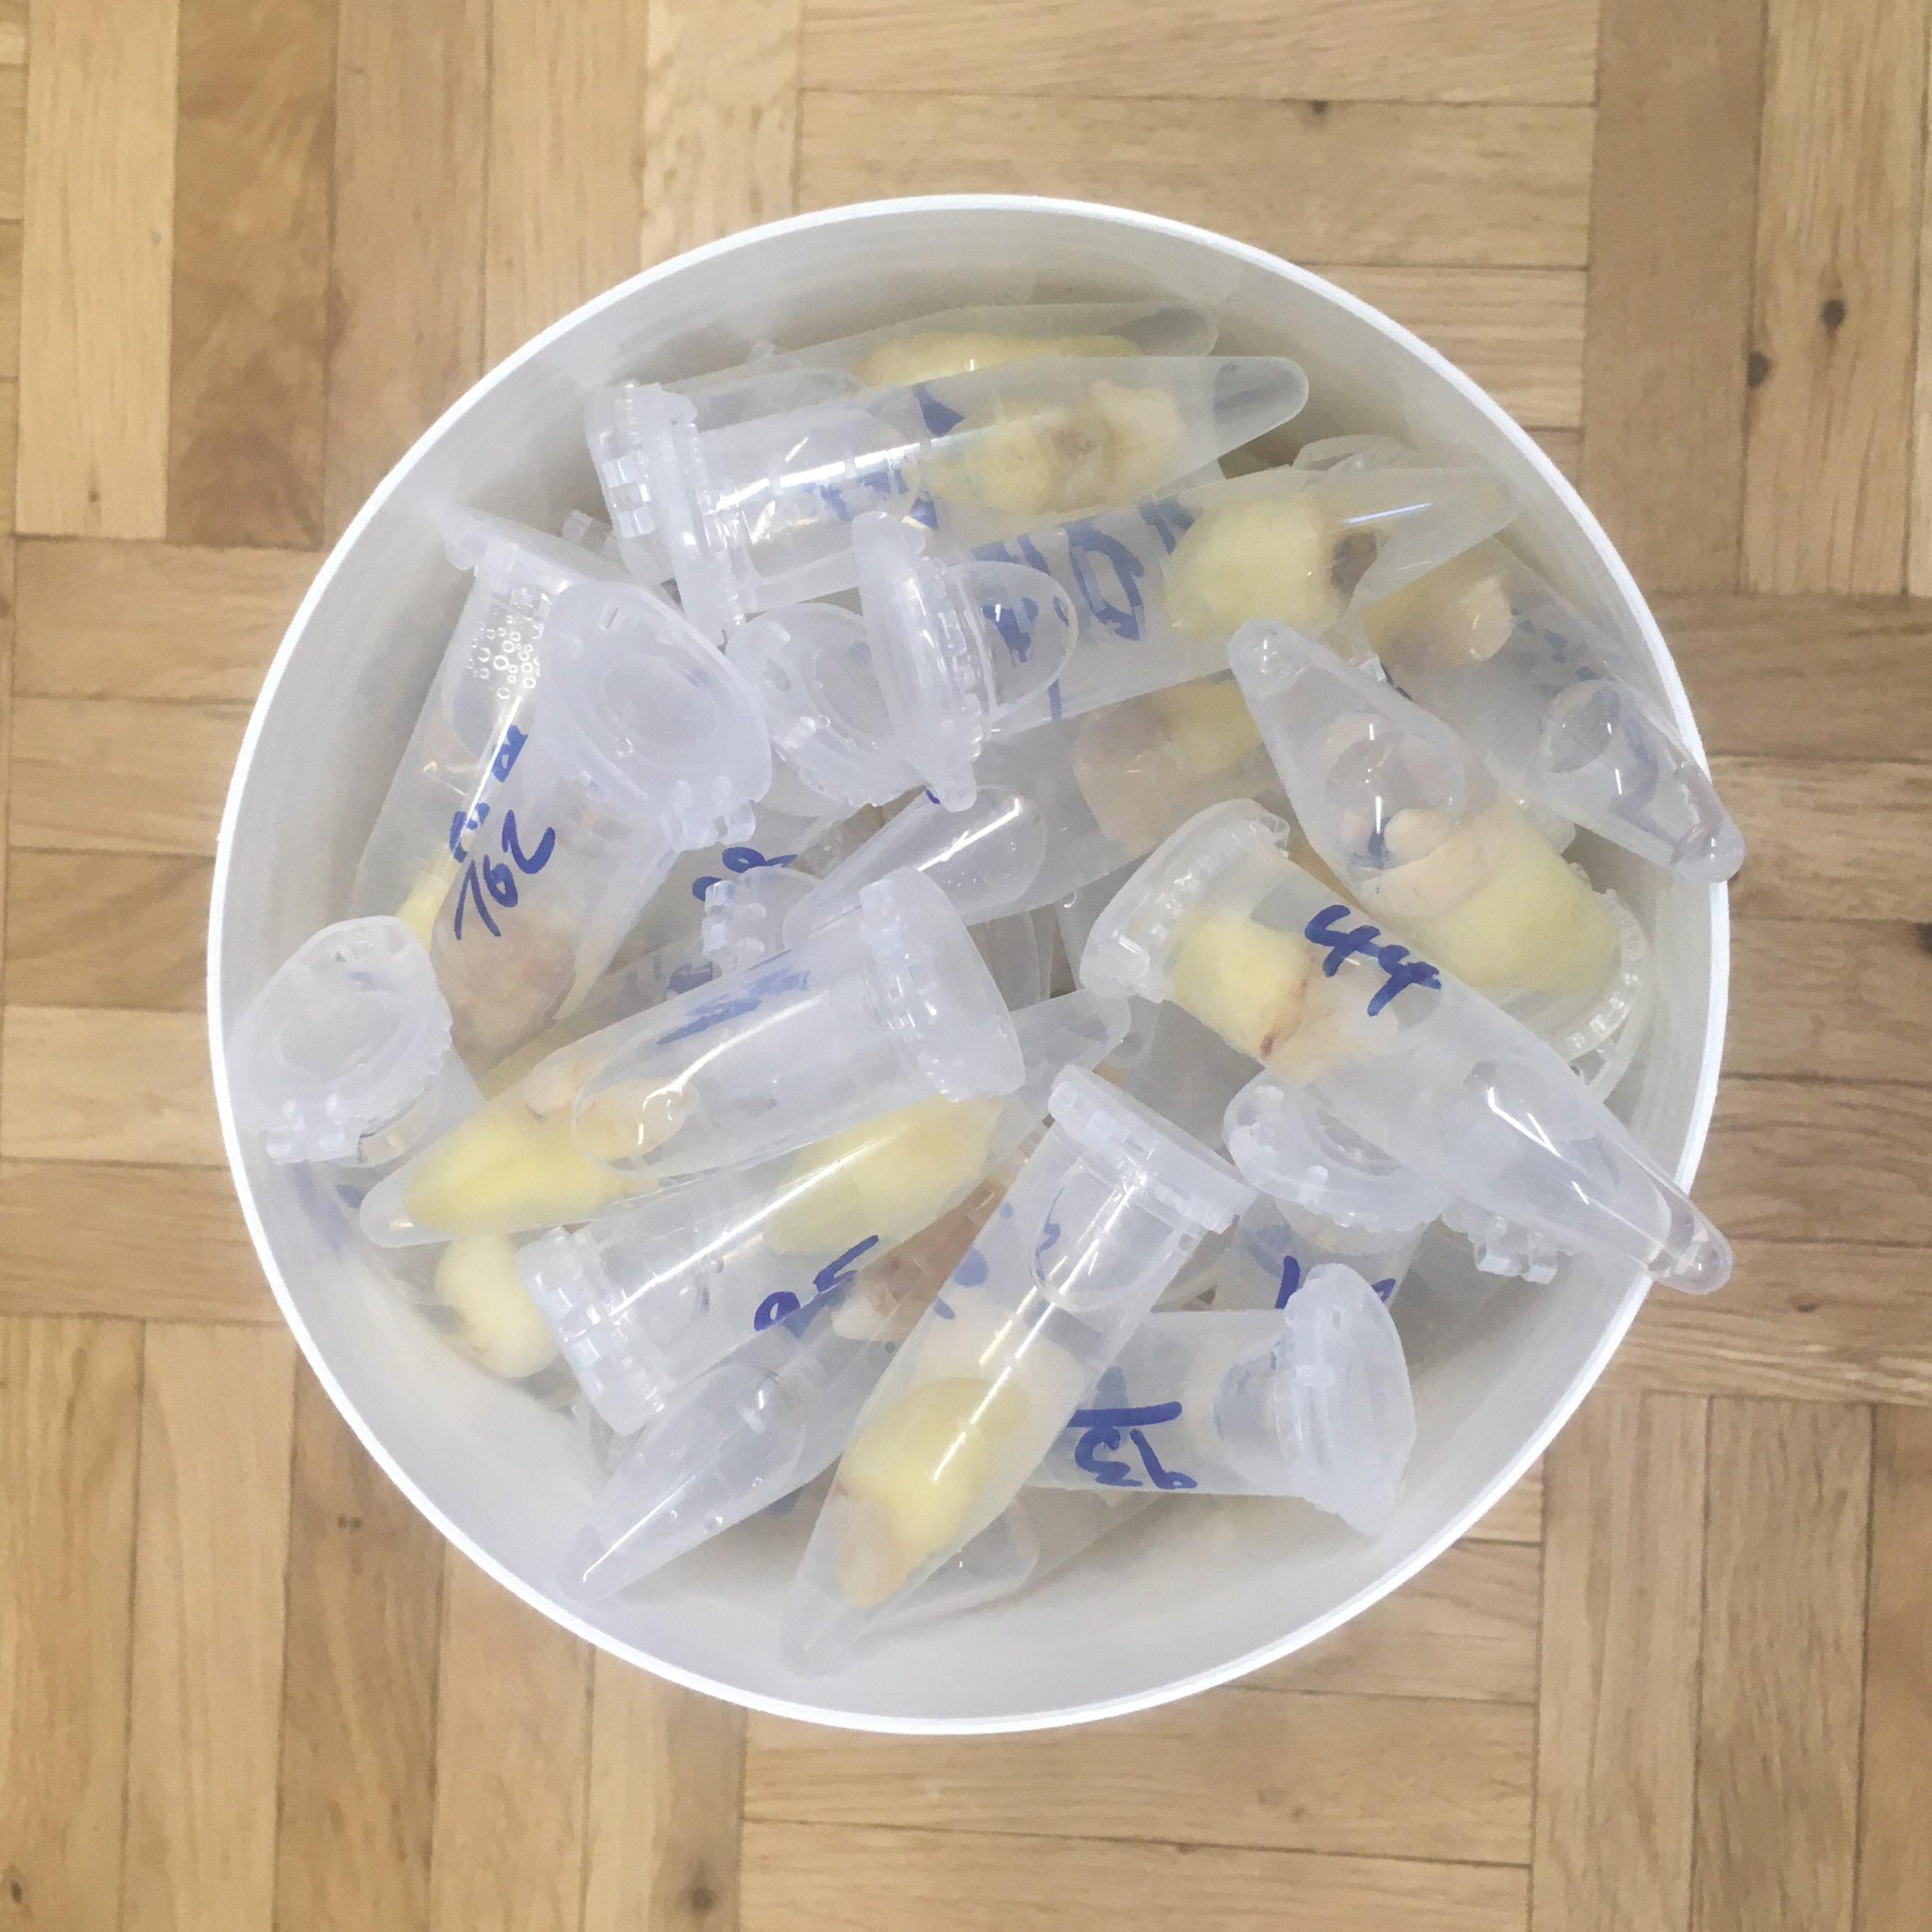
\includegraphics[width=\imagewidth]{./images/bucketofteeth}};
				% 2132.087px = 140.0mm -> 100px = 6566.337um -> 7.615px = 500um, 1.523px = 100um
				%\draw[|-|,blue,thick] (299,1340) -- (2430,1406) node [sloped,midway,above,fill=white,semitransparent,text opacity=1] {\SI{140.0}{\milli\meter} (2132px) TEMPORARY!};
				\draw[|-|,white,thick,shadowed] (\x,\y) -- (\x+761.5,\y) node [midway,above] {\shadowtext{\SI{5}{\centi\meter}}};
			\end{tikzpicture}%
			}%
			\renewcommand{\imagewidth}{\columnwidth}
		\end{column}%
	\end{columns}%
 \only<2>{
		\begin{tikzpicture}[remember picture,overlay]%
		\node at (current page.center) [shift={(0,-25pt)}]{%
		\animategraphics[autoplay,loop,width=\paperwidth,every=\everyframe]{24}{./movies/tooth045/transparent-slices-rcs/image0}{000}{457}%
			};%
	 \end{tikzpicture}%
	 }
\end{frame}

\section{Cichlids}
\begin{frame}
	\frametitle{Many more teeth, but from Cichlids}
		\begin{columns}
			\begin{column}{0.5\linewidth}
				\begin{itemize}
					\item Collaboration with team of \href{https://www.aqua.iee.unibe.ch/}{\emph{Aquatic Ecology \& Evolution}}, from the \href{https://www.iee.unibe.ch/}{Institute of Ecology and Evolution}
					\item 133 Cichlids from Lake Victoria, East Africa, to understand the functional anatomy of their skulls and jaws
					\begin{itemize}
						\item 375 scans in total
						\item 46 days of scanning time
						\item \qty{9.8}{\tera\byte} of raw data
						\item \qty{1.5}{\tera\byte} of reconstructions
						\item +\num{1000000} images
					\end{itemize}
				\end{itemize}
			\end{column}
			\begin{column}{0.5\linewidth}
				\centering
				\only<1>{%
					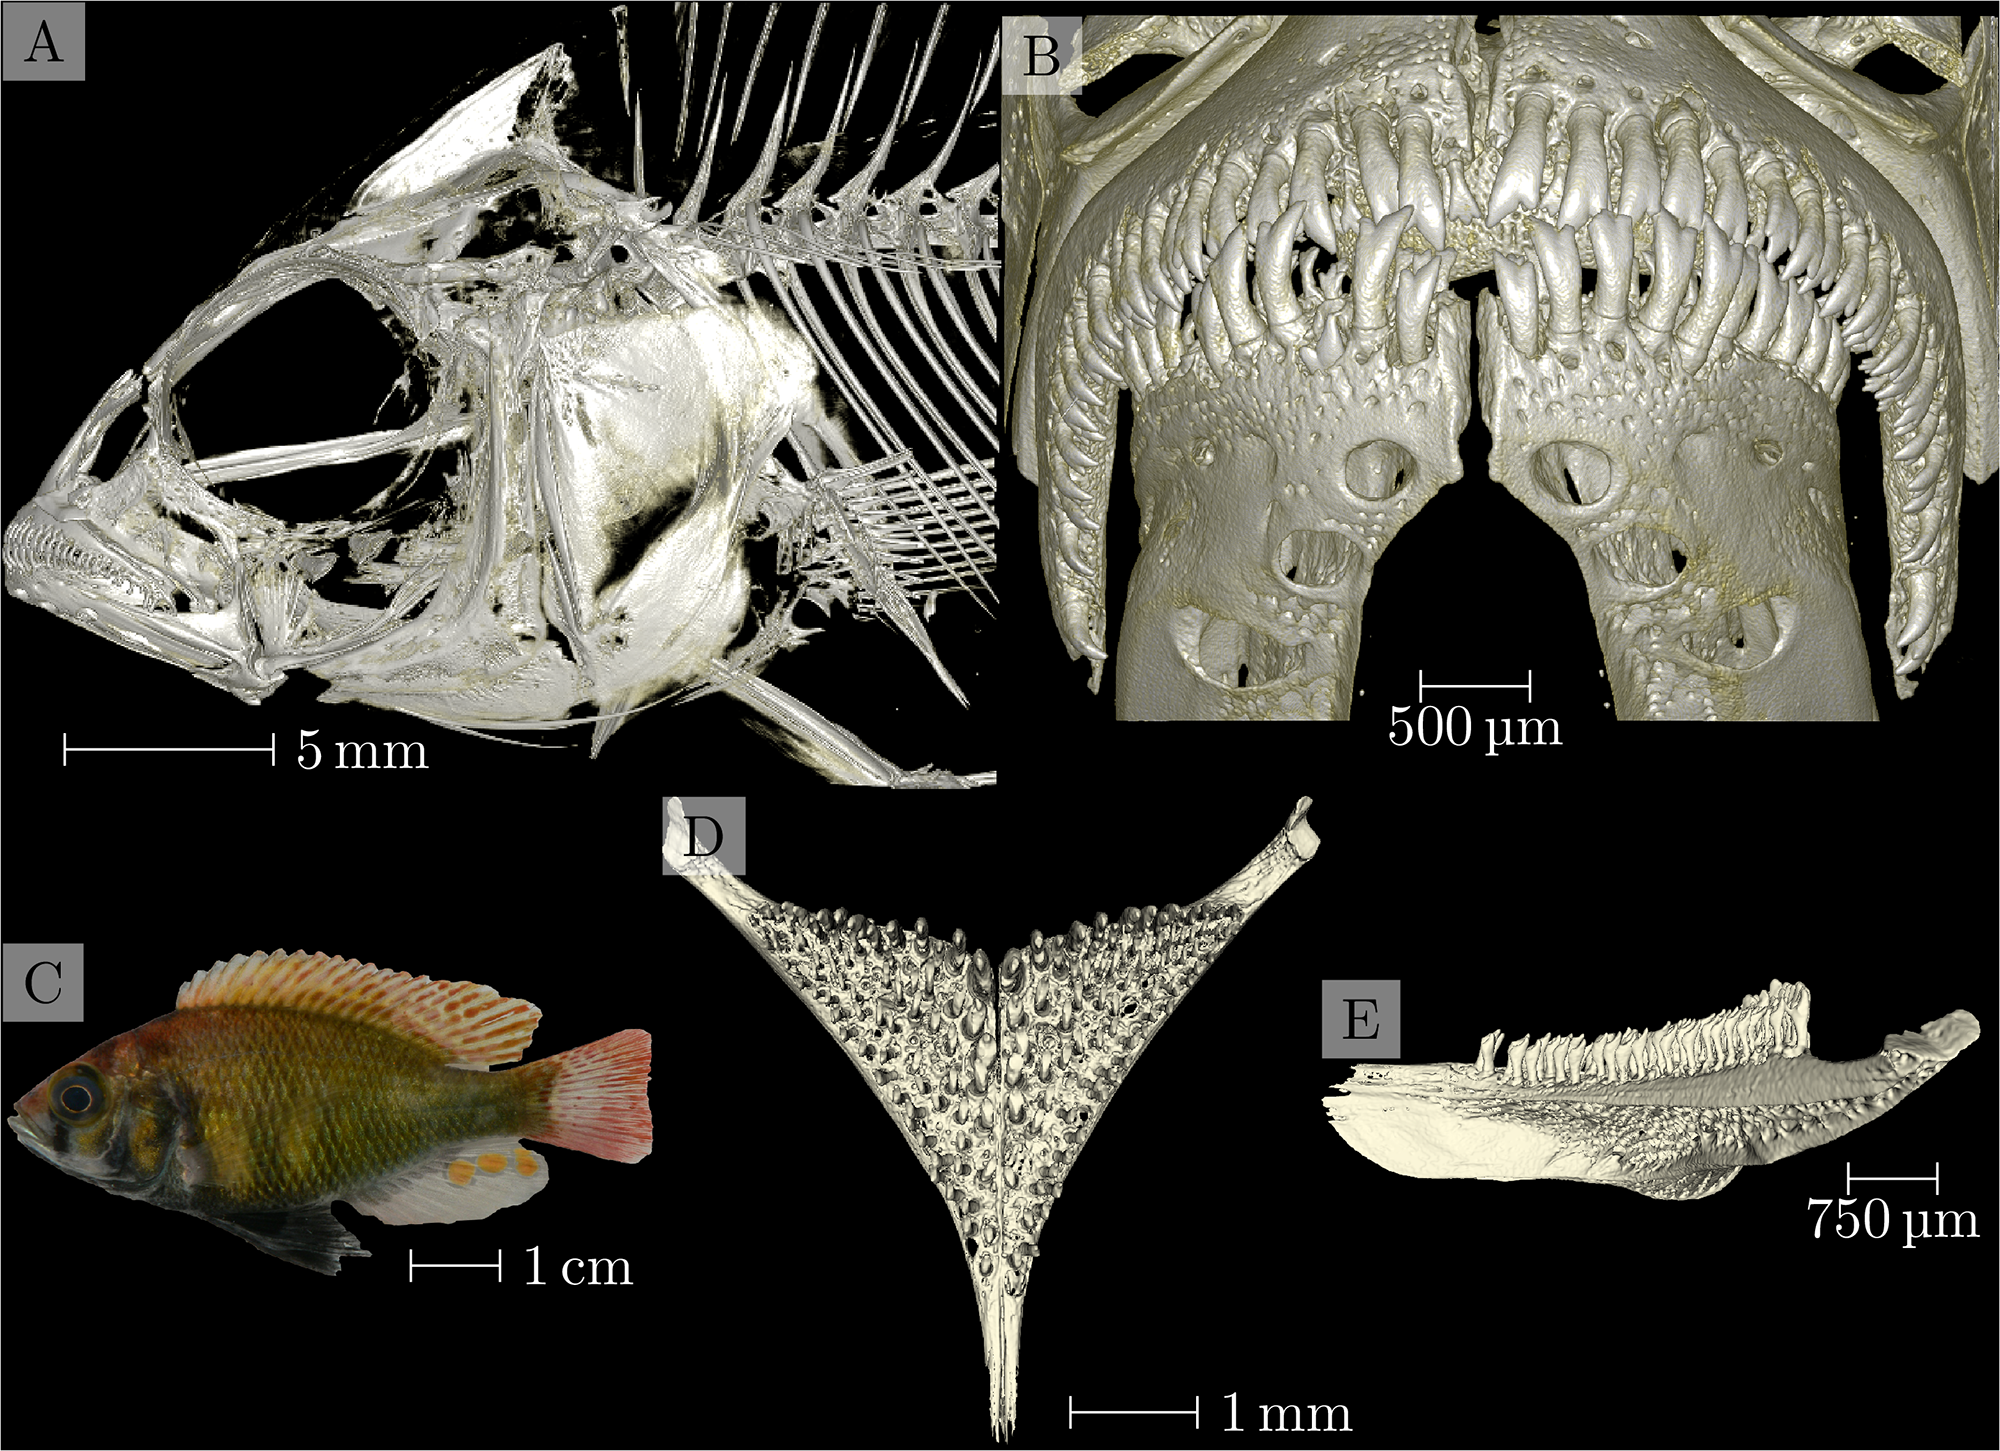
\includegraphics[width=\imagewidth]{./images/EAWAG/journal.pone.0291003.g001.png}%
					\sourcelink{https://journals.plos.org/plosone/article/figure?id=10.1371/journal.pone.0291003.g001}{doi:10.1371/journal.pone.0291003}{Fig.~1}%
					}%
				\includegraphics<2>[width=\imagewidth]{./images/EAWAG/lengths.plot.png}%
				\includegraphics<3>[width=\imagewidth]{./images/EAWAG/lengths.violinplot.png}%
				\includegraphics<4>[width=\imagewidth]{./images/EAWAG/lengths.boxplot.png}%
				\includegraphics<5>[width=\imagewidth]{./images/EAWAG/lengths.boxenplot.png}%
				\includegraphics<6>[width=\imagewidth]{./images/EAWAG/lengths.boxenplot.only.png}%
			\end{column}
		\end{columns}
\end{frame}

\begin{frame}
	\frametitle{Datasets}
		\animategraphics[autoplay,loop,height=\imageheight,every=\everyframe]{24}{./images/EAWAG/animation.intro/ 104016}{0000}{0050}%
\end{frame}

\section{cox7a}
\begin{frame}
	\frametitle{More fish, but muscles}
	\begin{itemize}
		\item Collaboration with \emph{Developmental Biology and Regeneration} group of Nadia Mercader Huber
		\item \footfullcite{Mercader2024}
	\end{itemize}
\end{frame}

\begin{frame}
	\frametitle{Volume plot}
\end{frame}

\begin{frame}[allowframebreaks]
	\frametitle{References}
	\renewcommand*{\bibfont}{\scriptsize}
	\setbeamertemplate{bibliography item}{\insertbiblabel}
	\printbibliography{}
\end{frame}

\end{document}
